\documentclass[a4paper,12pt]{article}
\usepackage[utf8]{inputenc} 
\usepackage[english,russian]{babel}
\usepackage{graphics}
\usepackage{epsfig}
\usepackage{amsmath,amssymb}

\title{Measurement of B($J/\psi \to K^+K^-$)/B($J/\psi \to \mu^+\mu^-$)
with BES-3 detector}
\author{I.B. Nikolaev}


\newcommand{\ee}{e^{+}e^{-}}
\newcommand{\uu}{\mu^{+}\mu^{-}}
\newcommand{\KK}{K^{+}K^{-}}
\newcommand{\pipi}{\pi^{+}\pi^{-}}

\begin{document}
\maketitle

\section{Introduction}

\section{Event selection}

At first stage of selection exactly four  charged which begin from interaction point tracks are selected:
\begin{itemize}
	\item $N_q = 4$
	\item $|z| <  10$~cm,  $r_{xy} < 1$~cm. Here $z$ is the distance from poca track to interaction point along axis z, 
		and $r_{xy}$ is the distance from poca track to interaction point in the xy-plane.
	\item $|\cos{\theta}|<0.8$, where $\theta$ is the polar angle of charged track.
\end{itemize}


Two opposite charged tracks with momentum less 0.45~GeV is considered to be
$\pi^+$- and $\pi^-$- mesons candidates. This pion pair must have recoil
invariant mass in the window from 3.0 to 3.2 GeV.
\begin{itemize}
	\item $p<0.45$~GeV
	\item $3.0 < M_{rec} < 3.2$ GeV
\end{itemize}

\begin{figure}
\begin{center}
  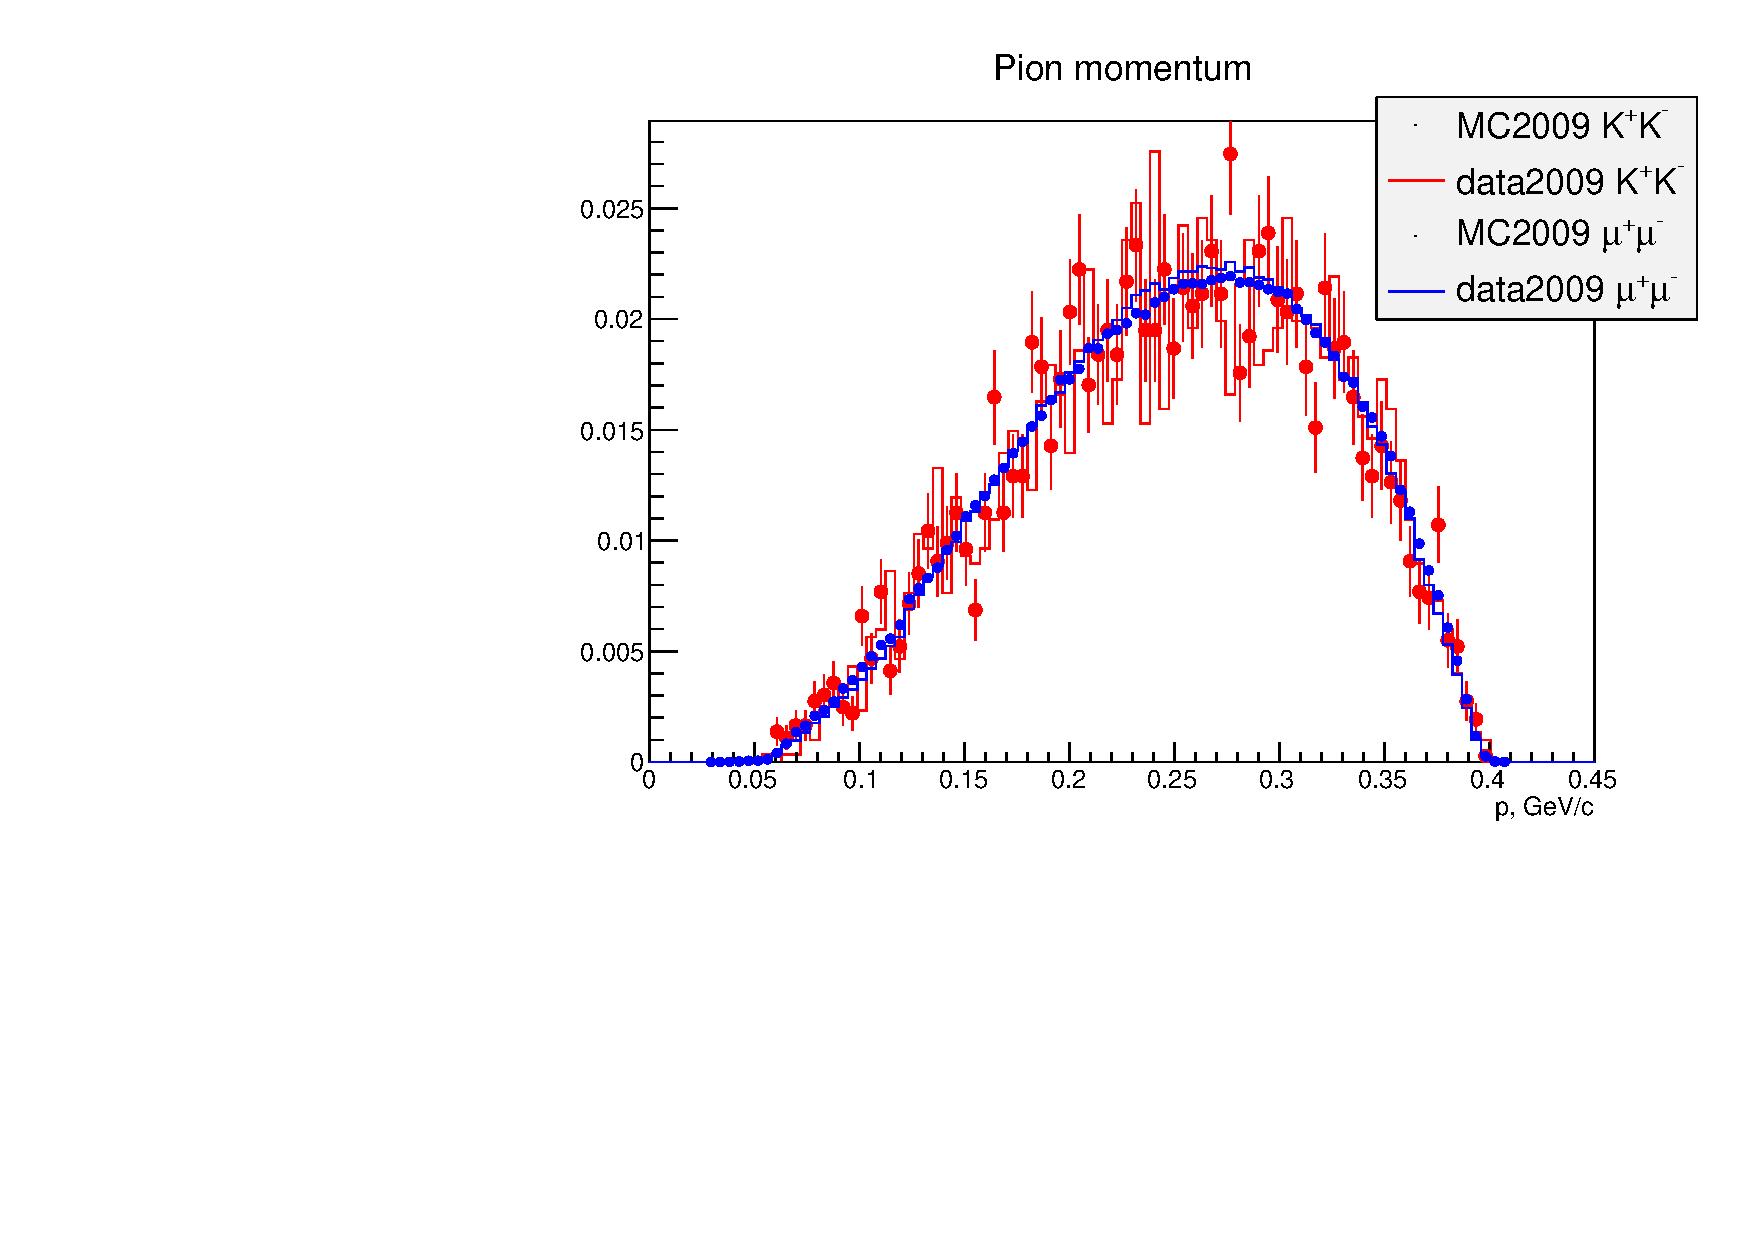
\includegraphics[width=0.5\textwidth]{fig/pion_momentum.pdf}
  \caption{Pion momentum cut $p<0.45$~GeV is used}
\end{center}
\end{figure}

Two other particles must be opposite charged and have momentum more then 1.0
GeV and less 2 GeV. To suppress $\ee$ background E/p ration must be less 0.8
GeV.
\begin{itemize}
	\item $1.0<p<2.0$~GeV
	\item $E/p < 0.8$~GeV
\end{itemize}

For this selected tracks vertex fit: all tracks must begin from single point.
Then kinematic fit was applied in two hypothesis for $\pi^+\pi^-\mu^+\mu^-$ and
$\pi^+\pi^-K^+K^-$ final state. 
\[
	P_{\psi(2S)} = P_{\pi^+} +  P_{\pi^-} + P_{K^+} +  P_{K^-}
\]

\[
	P_{\psi(2S)} = P_{\pi^+} +  P_{\pi^-} + P_{\mu^+} +  P_{\mu^-}
\]

here  $P_{\psi(2S)} = M_{\psi(2S)}\times (\sin(\alpha_{BEPC}/2),0,0, 1)$ ---
initial four momentum of $\psi(2S)$.  here $M_{\psi(2S)} = 3.686108\
\mbox{GeV}$ is the PDG-2014 mass of the $\psi(2S)$ resonance,
$\alpha_{BEPC}=0.022$ is the beam crossing of BEPC-II. Choose KK or $\mu\mu$
hypothesis corresponding lower $\chi^2_{kin}$. Addition information for
particle identification used for TOF and MDC DeDx system.
$\chi^2_{PID} = \chi^2_{TOF} + \chi^2_{dE/dx}$

For kaon case:
\begin{itemize}
	\item $\chi^2_{kin}{KK} <200$
	\item $\chi^2_{kin}(KK) < \chi^2_{kin}(\mu\mu)$
	\item $\chi^2_{pid}(KK) < \chi^2_{pid}(\mu\mu)$
	\item $\chi^2_{pid}(KK) < \chi^2_{pid}(\pi\pi)$
\end{itemize}


\begin{table}
	\begin{tabular}{lc} \hline
		process &  probability \\ 
		$\psi(2S) \to K_1^{\pm}(1270) K^{\mp}$  & $0.0005 \times 2$ \\ 
		$\psi(2S) \to K^+K^-\pi^+\pi^-$   & $7.5 \times 10^{-4}$  \\
		$\psi(2S) \to \rho^0 K^+K^-$   & $2.2 \times 10^{-4}$  \\
	$\psi(2S) \to  K^\pm \pi^\mp K^{*}(892)^0$  &  $6.7\pm10^{-4}$
	\end{tabular}
\end{table}


\begin{figure}
	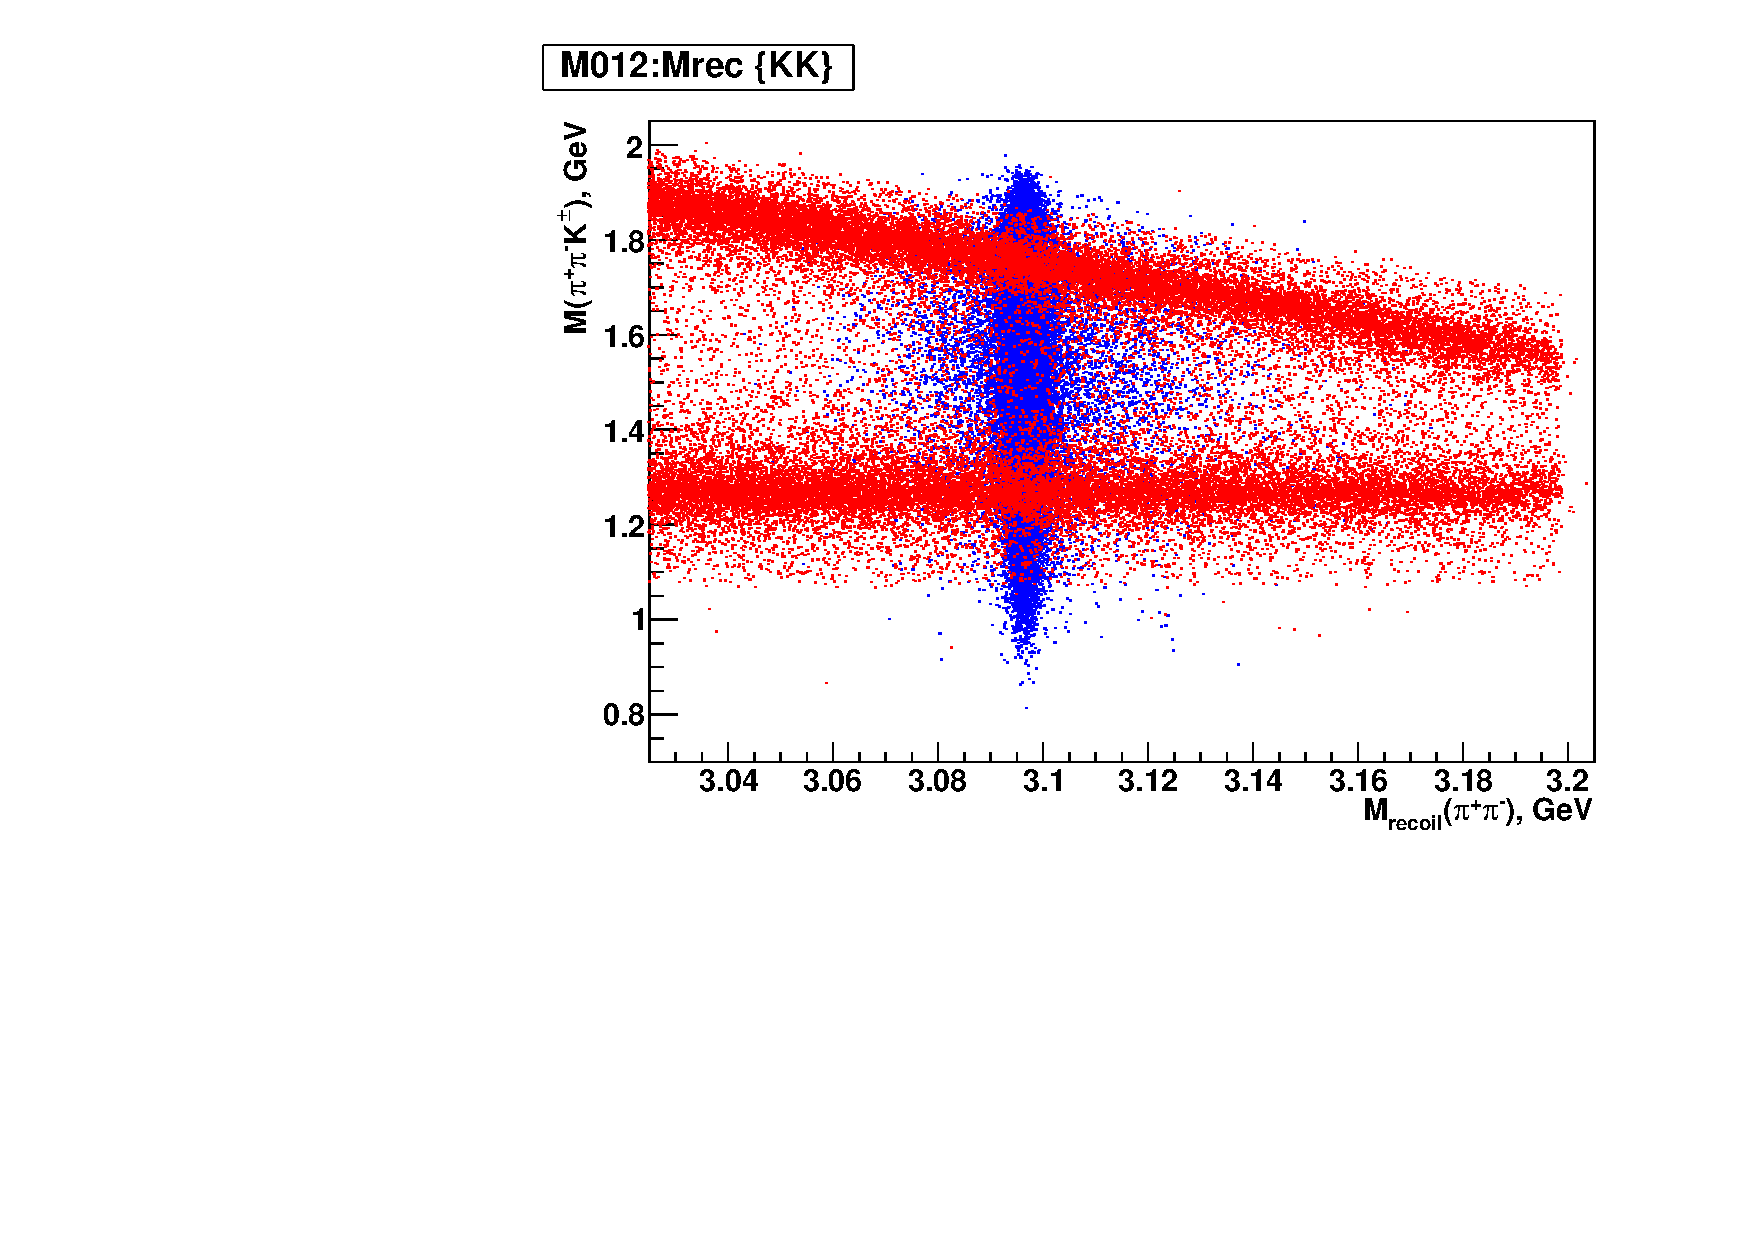
\includegraphics[width=\textwidth]{fig/M012_Mrec-color.pdf}
	\caption{Axis X -recoil invariant mass of $\pi^+\pi^-$,  axis y - invariant
	mass of $\pi^+\pi^-K^\pm$.  Blue is for $\psi^\prime \to J/\psi \pi^+\pi^-
	\to K^+K^-\pi^+\pi^-$. Red for $\psi^\prime \to K_1(1270)^\mp K^\pm  \to
	K^+K^-\pi^+\pi^-$}
\end{figure}


\subsection{Fit for recoil mass}

In order to fit $\pi^+\pi^-$ recoil mass modified Crystal Ball \cite{CrystalBallFunc}functin with right and left tail is used:
\begin{equation}
	%mCristalBall(x, N, \alpha_{el},\alpha_{l}, n_l,  \alpha_{er}, \alpha_r,  n_r )  = 	N \left\{
	f_{CB}(x)  = 	\left\{
		\begin{array}{lrrr}
			A_l(B_l - x)^{-n_l},  & -\infty &   x <&   -\alpha_l \\
			A_{el}\exp(\alpha_{el}x), &  -\alpha_l & < x  < &-\alpha_{el} \\
			\exp( - x^2/2),  &  - \alpha_{el} & < x < & \alpha_{er} \\
			A_{er}\exp(-\alpha_{er}x), &  \alpha_{el} & < x < & -\alpha_{r} \\
			A_r(B_r + x)^{-n_r}, &   \alpha_r & < x < & \infty \\
		\end{array}
		\right., 
\end{equation}
\begin{equation}
	\begin{array}{lcl}
		A_{er, el} & = &  \exp(\alpha_{er, el}^2/2) \\
		B_{ r, l}  &  = & n_{r, l}/ \alpha_{er, el} - \alpha_{r, l}
	\end{array}
\end{equation}


Fit function is
\begin{equation}
N f_{CB}\left( \frac{m - M}{\sigma},  \alpha_{el},\alpha_{l}, n_l,  \alpha_{er}, \alpha_r,  n_r\right)  +  N_{bg}
\end{equation}








\begin{figure}
	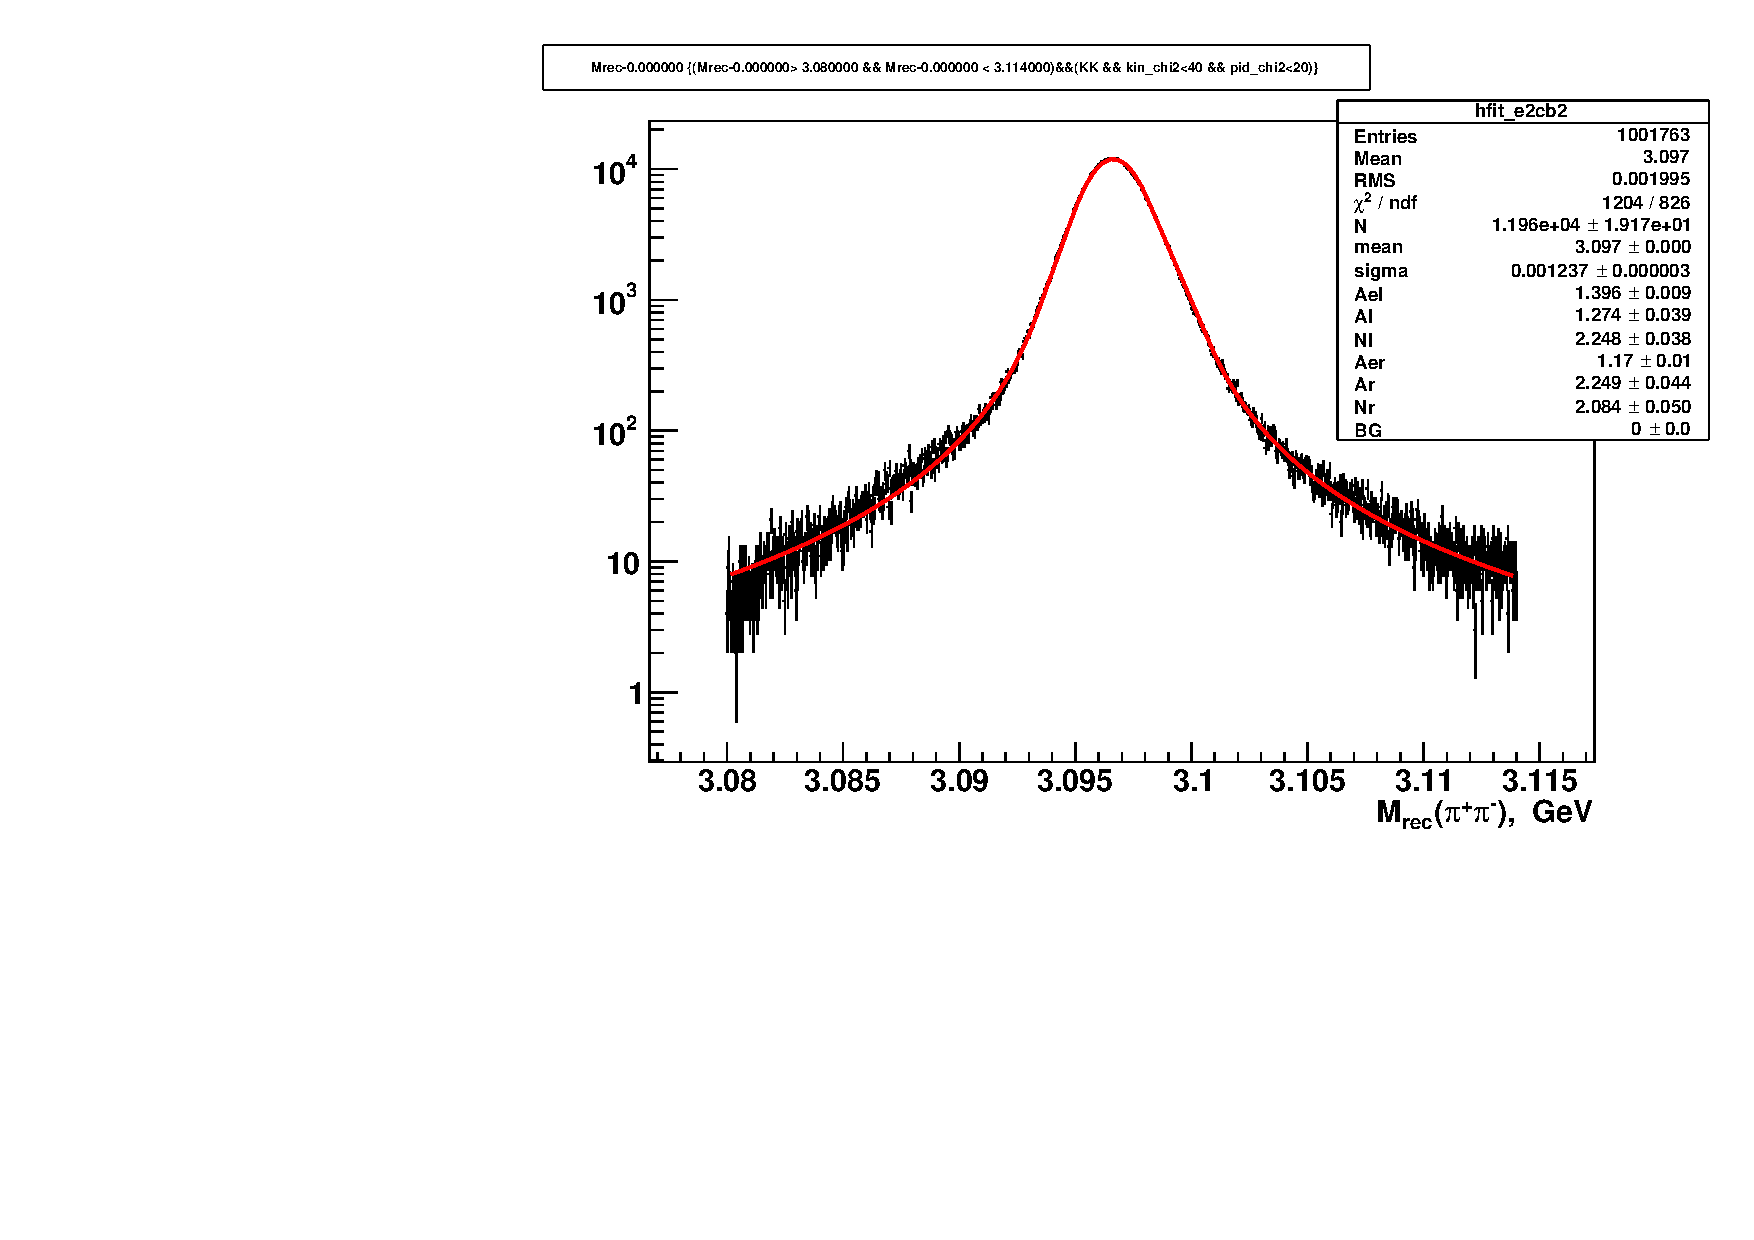
\includegraphics[width=\textwidth]{fig/Mrec_fit_double_exp_double_crystal_ball.pdf}
	\caption{Recoil invariant mass of $\pi^+\pi^-$ fitted by 
		modified Crystall Ball function}
\end{figure}

\end{document}

